\section{Aktuator Design (Henrik og Morten)}

Dette afsnit omhandler design af blokken Aktuator. Den opdeles i underblokkene Varmelegeme, Blæsere, Vinduesmotor og PSoC4.

\subsection{Varmelegeme}

\begin{figure}[h]
\centering 
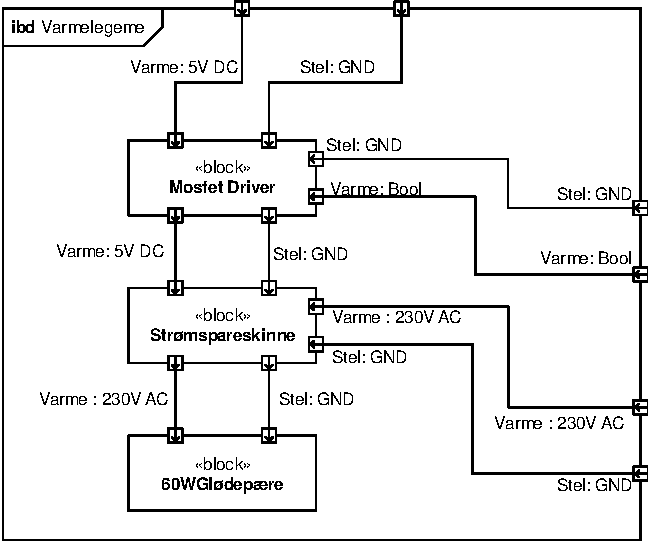
\includegraphics[width={\textwidth-5cm}, trim=0 0 0 0, clip=true] {../fig/ibd_varmelegeme.pdf}
\caption{IBD for underblokken Varmelegeme i Aktuator}
\label{fig:ibd_varmelegeme}
\end{figure}

Ovenstående diagram (Figur \ref{fig:ibd_varmelegeme}) viser interne forbindelser i underblokken Varmelegeme i Aktuator. 
For at undgå håndtering af 230V AC, består underblokken af en USB strømspareskinne, så selve varmelegemet (1-3 stk. 100W Glødepære) kan tændes og slukkes med et 5V DC signal. 
Antallet af tilkoblede glødepærer bestemmes under senere tests.

Aktuatorens SW er designet således at der nemt kan opgraderes til PWM styring af varmelegemet. 
Dette viser sig desværre at være umuligt med denne opstilling, da USB strømspareskinnen indeholder et mekanisk relæ; det er ikke muligt at opnå en frekvens hvor lyset ikke blinker. 
Dette vil sandsynligvis resultere i en sprunget glødepære.
En mulig løsning på problemet kunne være at tænde og slukke de 230V AC direkte med Mosfet transistoren, men vi må ikke håndtere så høje spændinger. 
En anden mulig løsning er at anvende for eksempel 12V glødepærer i stedet. Der skal dog nok temmelig mange til for at opnå samme effekt. 

Såfremt det senere vælges at opgradere til PWM styring, skal man tage højde for - eller se bort fra - at effekten ikke er lineært sammenhængende med dytucyclen. Dette skyldes dels at effekt har en sammenhæng med kvadratet af strømmen, dels at modstanden i glødetråden afhænger af temperaturen. 

\clearpage

\begin{figure}[h]
\centering 
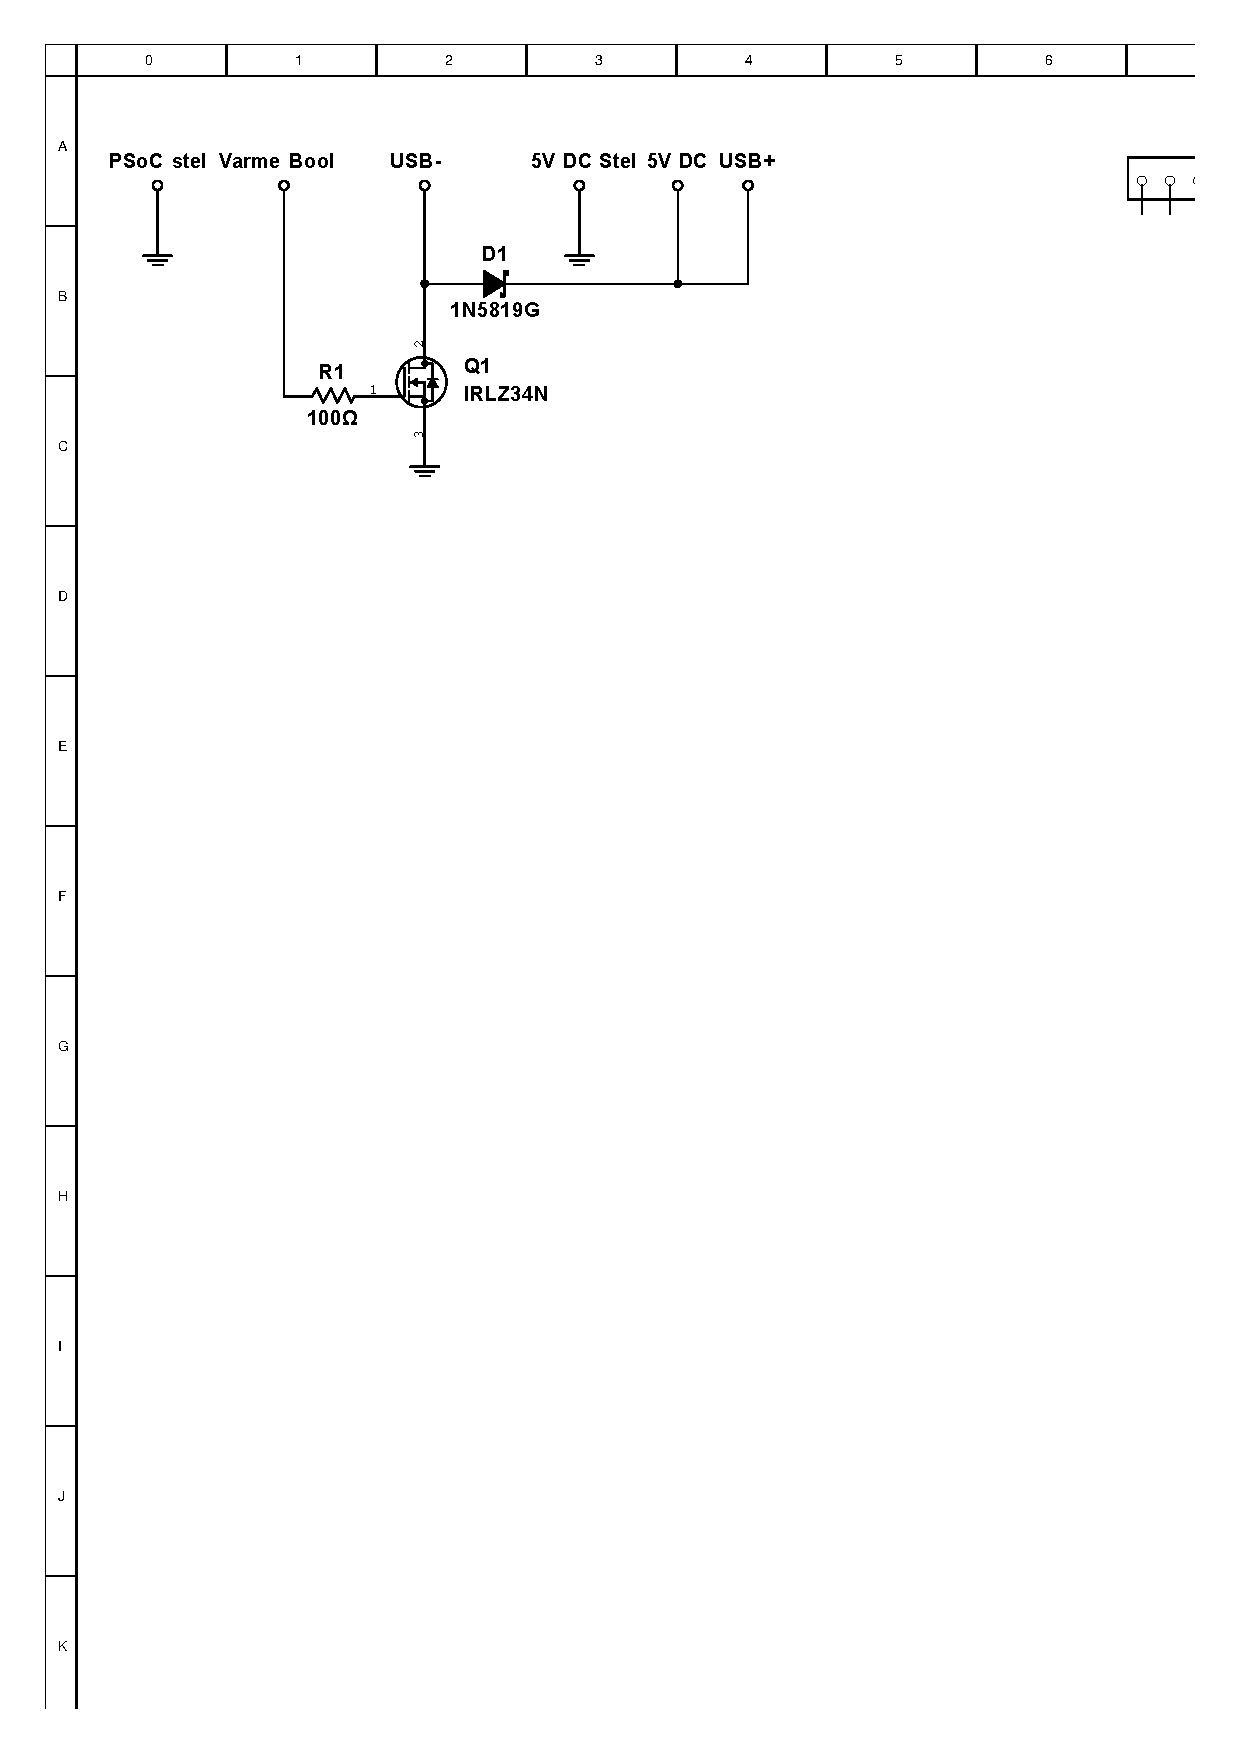
\includegraphics[width={\textwidth-5cm}, trim= 50 610 220 70, clip=true] {../fig/multisim_varmelegeme_mosfetdriver.pdf}
\caption{Kredsløb for Mosfet Driver i underblokken Varmelegeme}
\label{fig:multisim_varmelegeme_mosfetdriver}
\end{figure}

Når Varme Bool på Figur \ref{fig:ibd_varmelegeme} går høj, lukker mosfet transistoren, og tilslutter derved stel til USB Strømspareskinnen; varmelegemet forsynes med 230V AC. 
Når Varme Bool går lav, åbner mosfet transistoren, og derved afbrydes stel til Strømspareskinnen; varmelegemet forsynes ikke.  

D1 er er indsat for at sikre transistoren mod peakspændinger fra USB skinnen, når den slukkes. Dette er sandsynligvis ikke nødvendigt, men da vi ikke har indblik i hvordan USB strømspareskinnen rent faktisk virker, er dioden indsat for en sikkerheds skyld. 

Modstanden R1 er en beskyttelsesmodstand, som beskytter PSoC4, hvis Mosfet transistoren brændes af. 

\clearpage

\subsection{Blæsere}

\begin{figure}[h]
\centering 
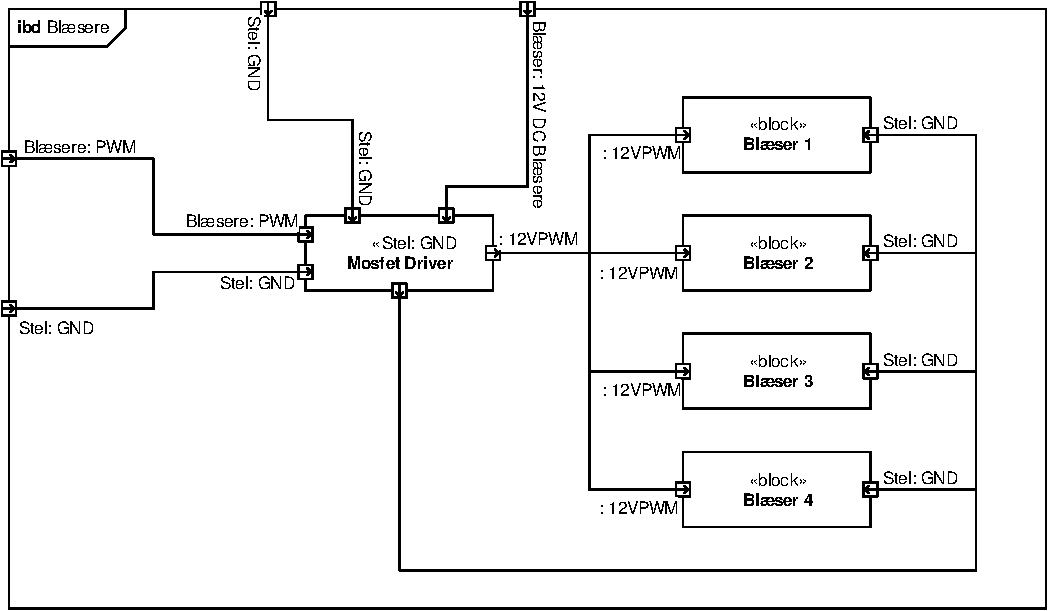
\includegraphics[width={\textwidth}, trim=0 0 0 0, clip=true] {../fig/ibd_blaesere.pdf}
\caption{IBD for underblokken Blæsere i Aktuator}
\label{fig:ibd_blaesere}
\end{figure}

Figur \ref{fig:ibd_blaesere} viser interne forbindelser i underblokken Blæsere, der består af en Mosfet Driver og fire 12V blæsere. 
To af blæserne er monteret således at luft blæses ind i drivhuset, mens de to øvrige blæsere blæser luft ud af drivhuset. 
Det forventes at en dutycycle på 100\% udskifter al luft i drivhuset på meget kort tid; dutycyclen for 'tændte blæsere' bestemmes ved praktiske forsøg under realisering af underblokken. 

Ved praktiske forsøg, konstateredes det, at en dutycyce på 50\% er et fornuftigt maximum. Det konstateredes desuden, at blæserne skal startes på maximum (dutycycle 50\%) for at komme i gang. 
Hvis der startes med en mindre dutycycle, opnår motoren ikke inerti nok til at begynde dreje. 
Begge dele implementeres i SW. 

\clearpage
 
\begin{figure}[h]
\centering 
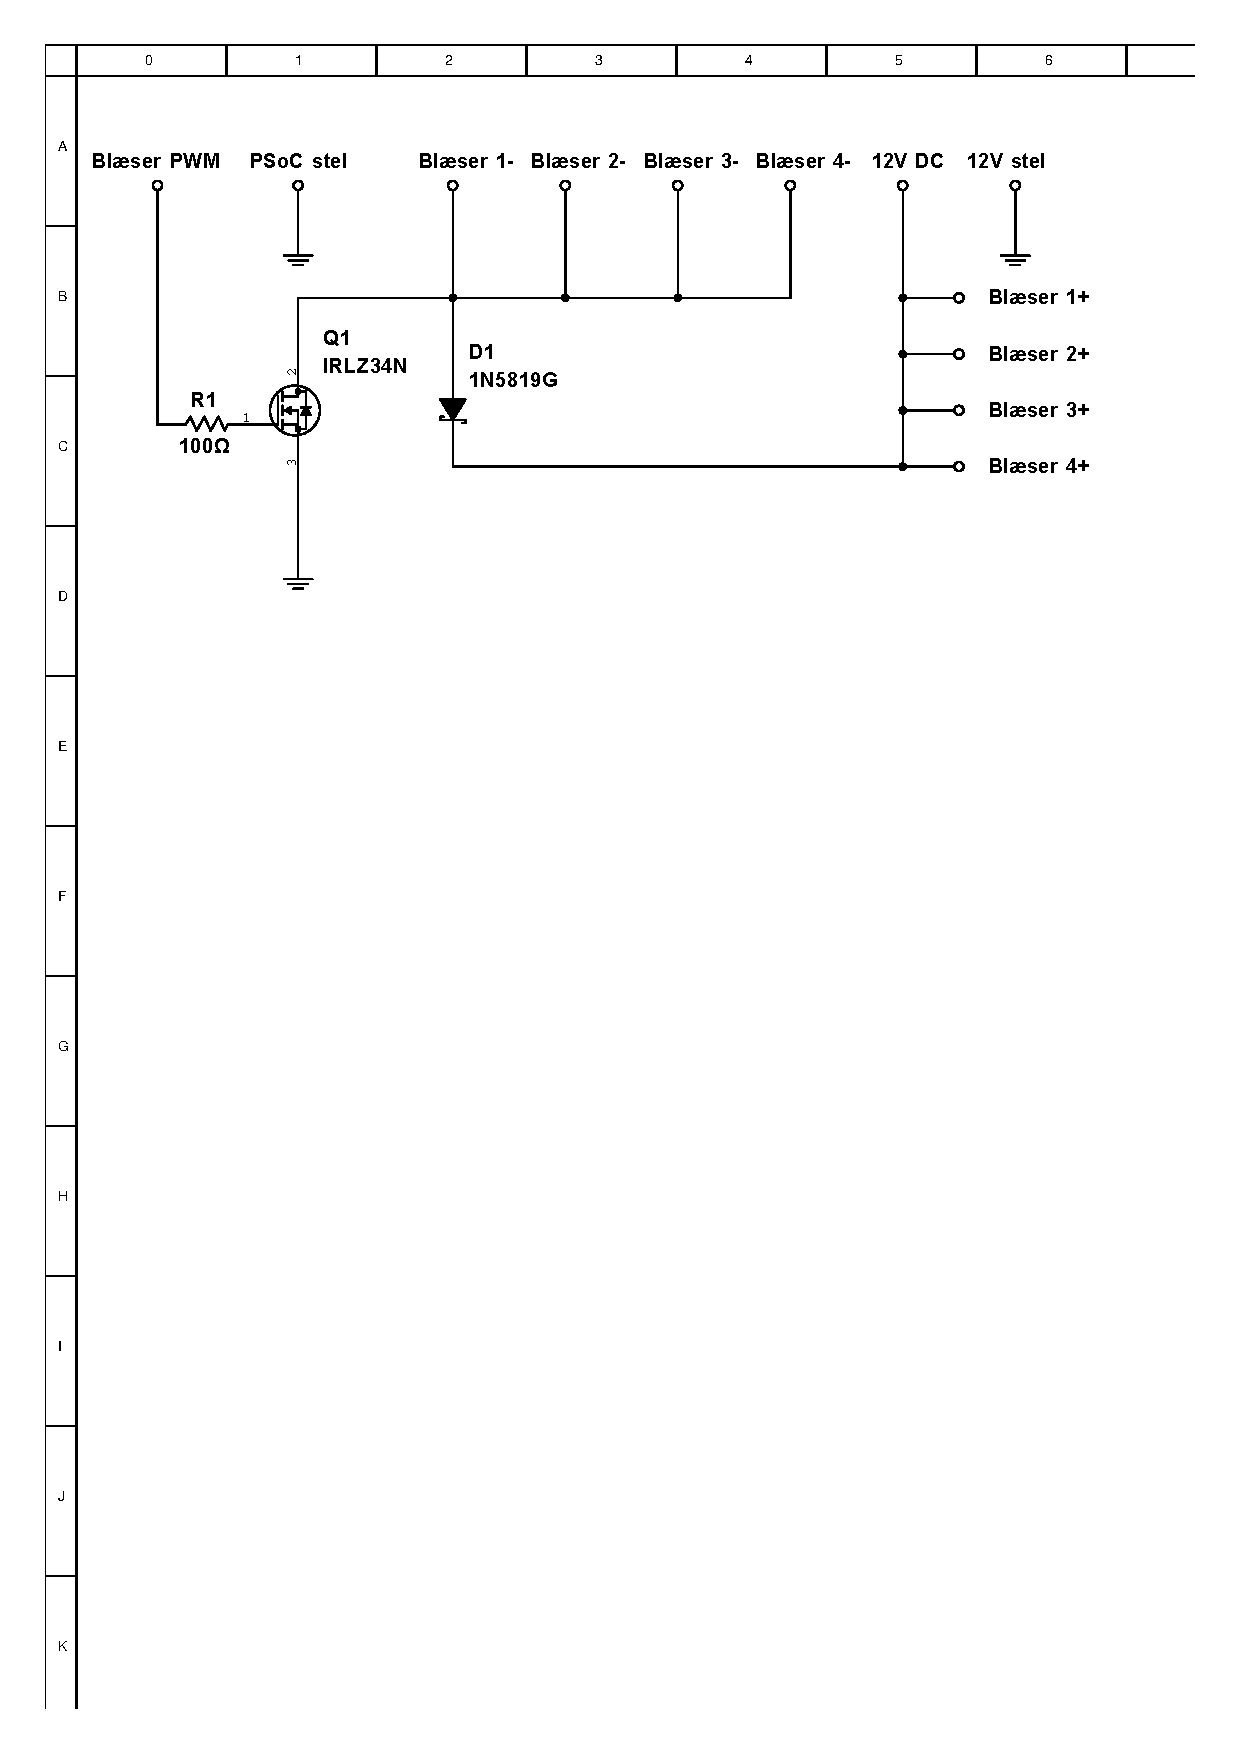
\includegraphics[width={\textwidth}, trim= 40 550 70 70, clip=true] {../fig/multisim_blaesere_mosfetdriver.pdf}
\caption{Kredsløb for Mosfet Driver i underblokken Blæsere}
\label{fig:multisim_blaesere_mosfetdriver}
\end{figure}

Mosfet Driveren til Blæsere på Figur \ref{fig:multisim_blaesere_mosfetdriver} fungerer i princippet på samme måde som Mosfet Driver for Varmelegeme (Figur \ref{fig:multisim_varmelegeme_mosfetdriver}).
Der er blot tilsluttet fire blæsere, der alle styres vha. den samme transistor. 

\clearpage

\subsection{Vinduesmotor}

\begin{figure}[h]
\centering 
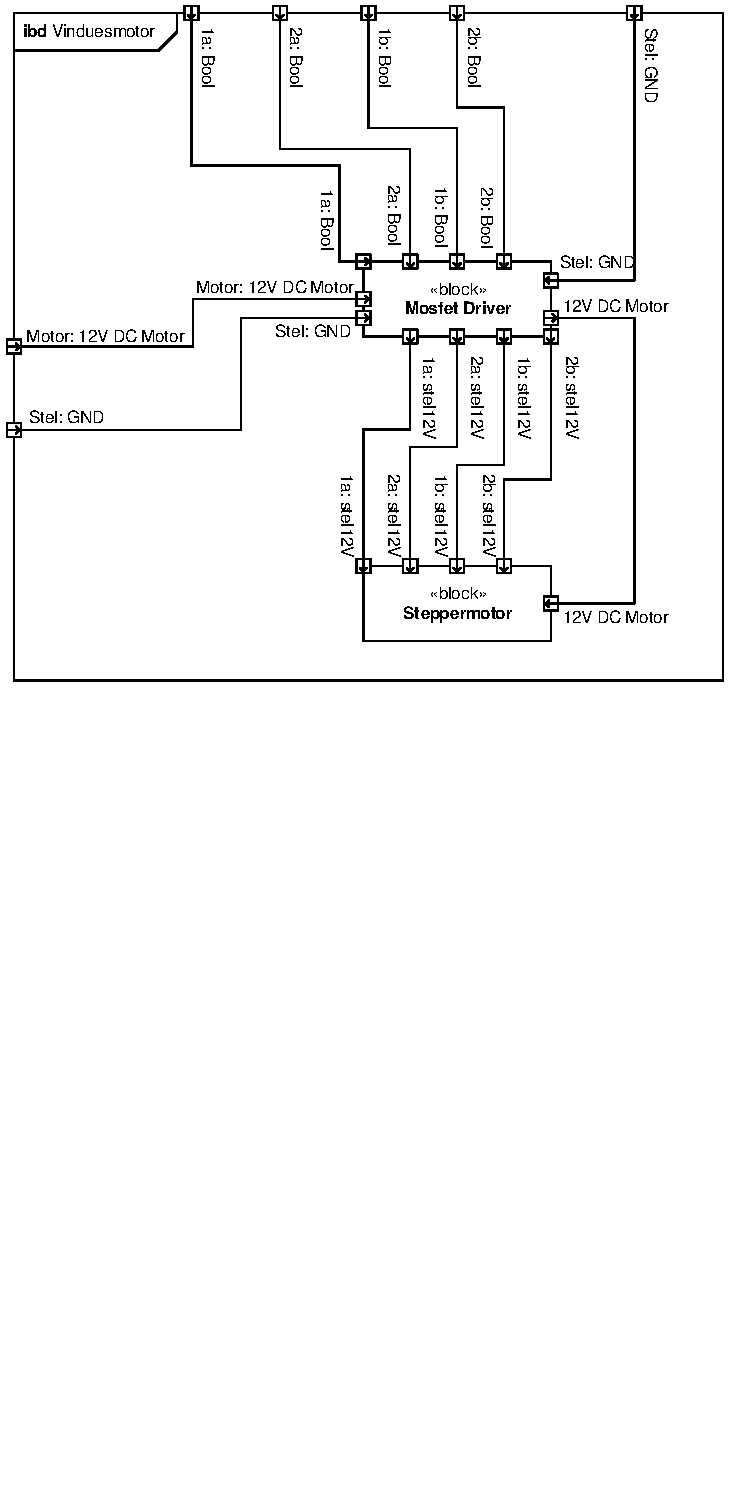
\includegraphics[width={\textwidth}, trim=0 390 0 0, clip=true] {../fig/ibd_vinduesmotor.pdf}
\caption{IBD for underblokken Vinduesmotor i Aktuator}
\label{fig:ibd_vinduesmotor}
\end{figure}

Ovenstående diagram (Figur \ref{fig:ibd_vinduesmotor}) viser interne forbindelser i underblokken Vinduesmotor, der består af en Steppermotor og en Mosfetdriver. 
Der åbnes og lukkes for mosfet transistorer i Mosfet Driveren vha. 3,3V signaler fra PSoC4, og derved forsynes Steppermotor med 12V DC. 
\\\\
Mosfet Driveren til Vinduesmotor på Figur \ref{fig:multisim_vinduesmotor_mosfetdriver} side \pageref{fig:multisim_vinduesmotor_mosfetdriver} fungerer i princippet på samme måde som Mosfet Driver for Blæsere (Figur \ref{fig:multisim_blaesere_mosfetdriver}).
Der er dog den forskel, at de fire signaler styres af hver deres transistor, da de ikke alle skal åbne og lukke samtidigt. 

\begin{figure}[h]
\centering 
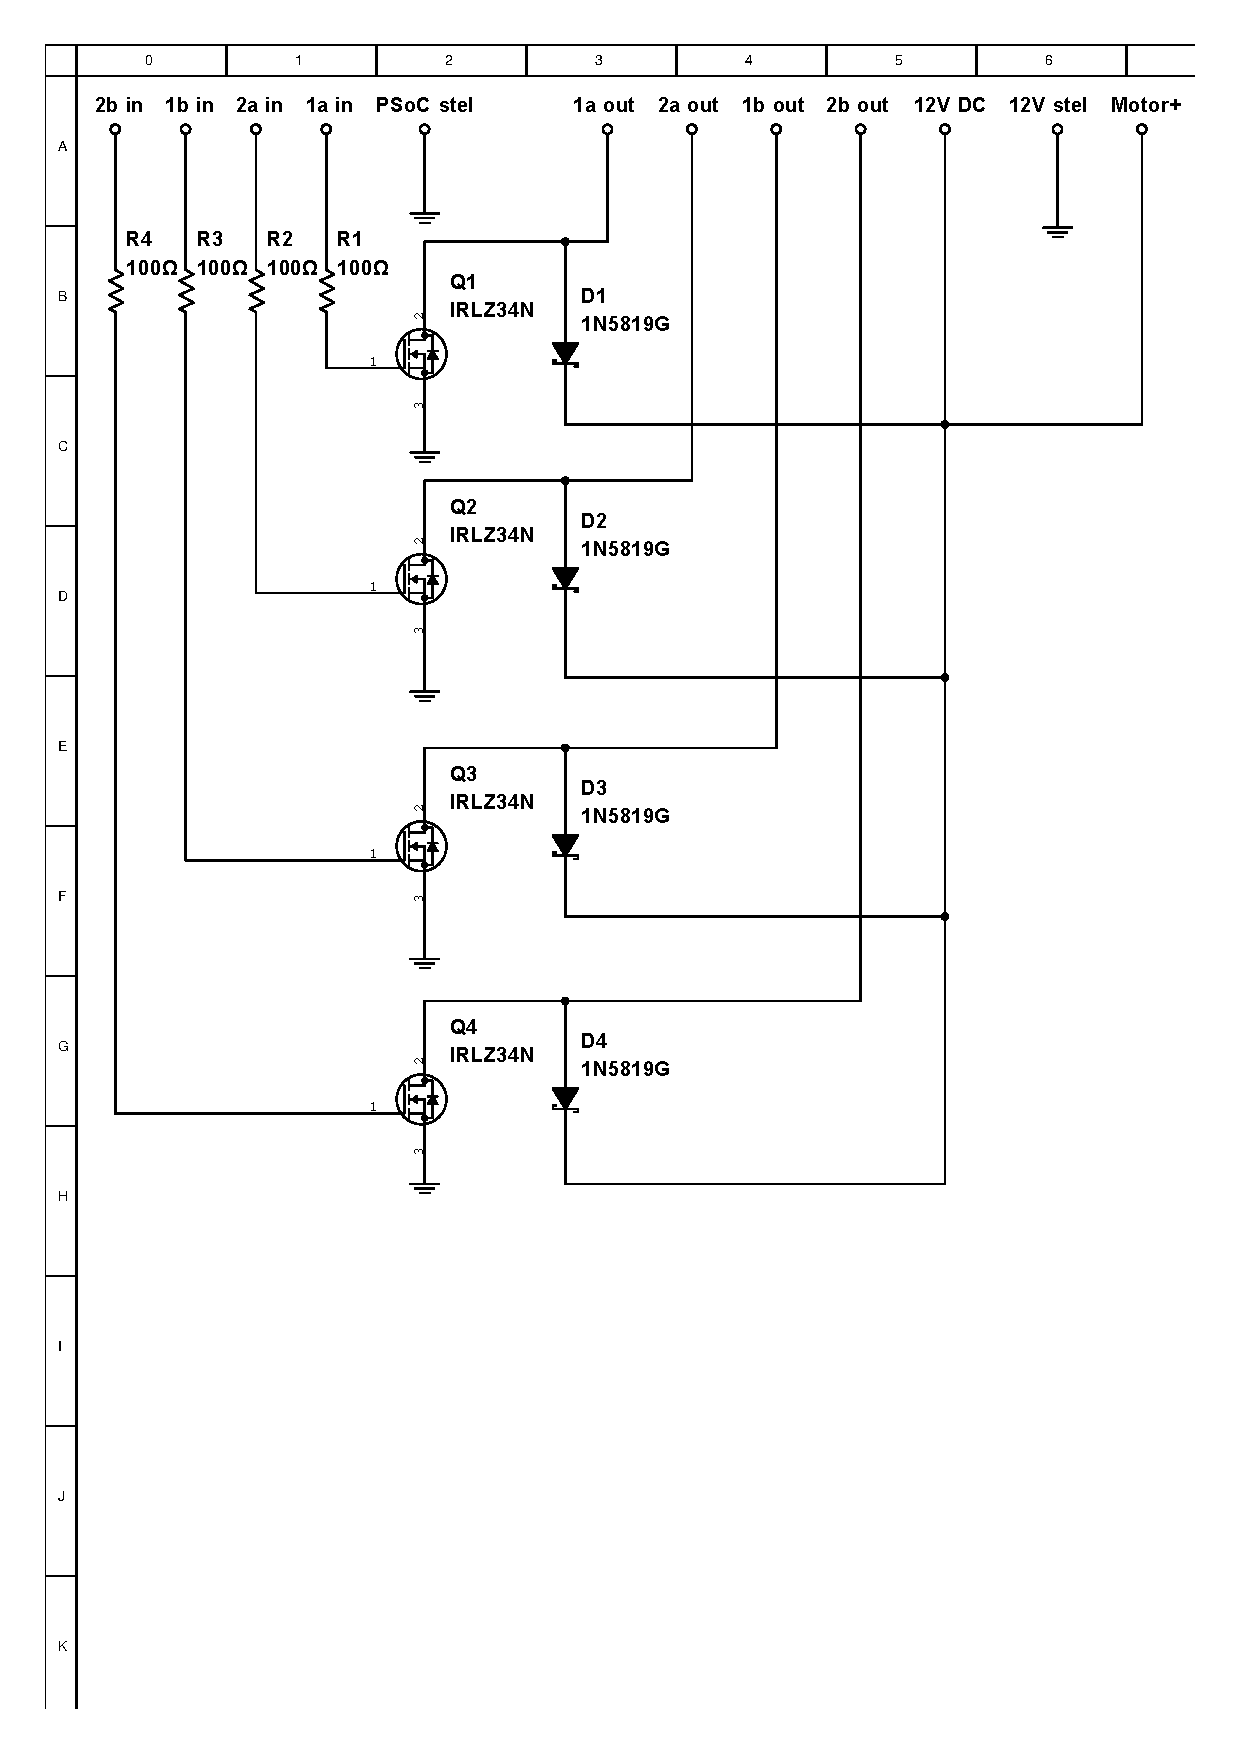
\includegraphics[width={\textwidth}, trim= 40 260 0 40, clip=true] {../fig/multisim_vinduesmotor_mosfetdriver.pdf}
\caption{Kredsløb for Mosfet Driver i underblokken Vinduesmotor}
\label{fig:multisim_vinduesmotor_mosfetdriver}
\end{figure}

\clearpage

\subsection{PSoC4}

\begin{figure}[h]
\centering 
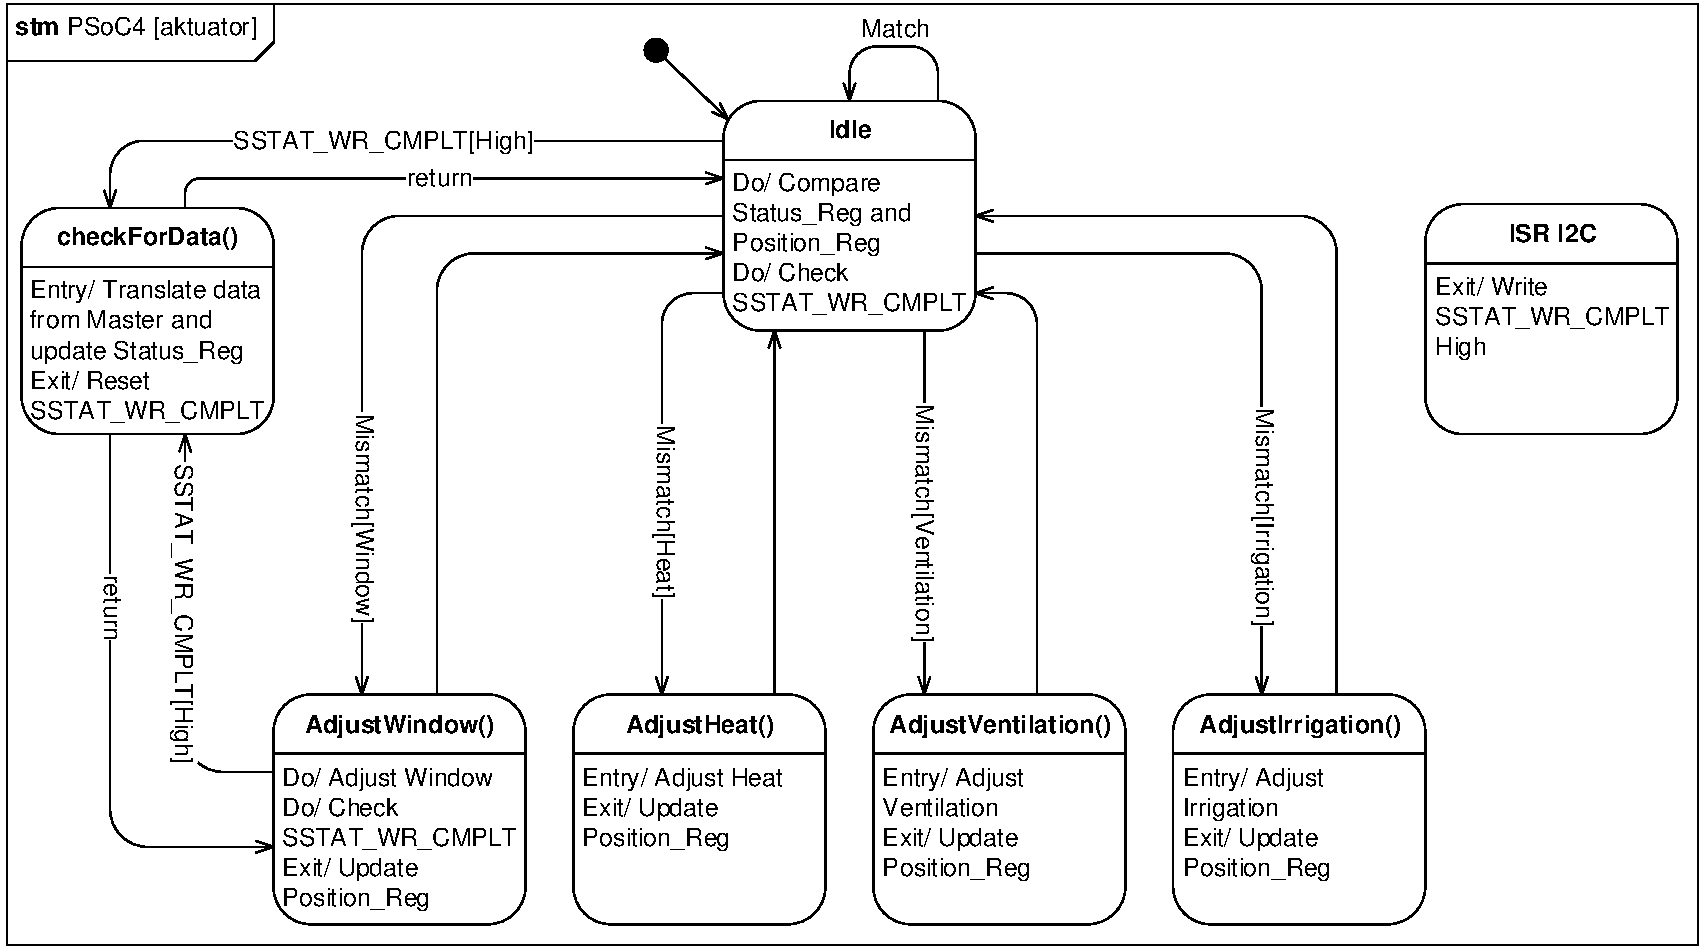
\includegraphics[width={\textwidth}, trim=0 0 0 0, clip=true] {../fig/stm_psoc_aktuator.pdf}
\caption{State Machine for software på underblokken PSoC4 i Aktuator}
\label{fig:stm_psoc_aktuator}
\end{figure}

Ovenstående diagram (Figur \ref{fig:stm_psoc_aktuator}) viser en state machine for software i underblokken PSoC4 i blokken Aktuator. 

Koden gentager tjek af om ønsket indstilling, af aktuatorer stemmer overens med aktuatorernes aktuelle indstilling og retter dette, såfremt det ikke er tilfældet. 
Denne rutine kan til enhver tid afbrydes af interrupt fra I2C bussen, der opdaterer slave write complete registeret (SSTAT\_WR\_CMPLT) fra lav til høj. Dette medfører at checkForData aktiveres som opdaterer ønskede indstillinger af aktuatorer. Herefter vil rutinen genoptages.
 
Ønskede indstillinger er gemt i registret Status\_Reg, mens aktuelle indstillinger er gemt i Position\_Reg.
 
Ved opdaterering af aktuatorer er den priorterede rækkefølge: Varme, blæsere, vanding og vindue. 
Vinduet er sidst i rækkefølgen, da det tager lang tid at åbne eller lukke. Koden for åbning eller lukning af vindue skrives således, at slave write complete registeret løbende tjekkes. Hvis dette register er højt vil indstillinger af aktuatorer opdateres, og derefter fortsætte fra vinduets position med de nye indstillinger.
Derved undgås det, at vinduet fx skal lukke helt, inden det åbnes, hvis disse to kommandoer modtages med meget kort mellemrum. 

\subsection{Drivers til PSoC4}
Dette afsnit beskriver drivere for opdatering af aktuatorer. 
Disse drivere er opdelt i Varme, Blæsere, Vanding, Vinduesmotor og checkForData. 
Derved kan systemet nemt opdateres, hvis der ændres på styringen af en bestemt aktuator. 
Alle drivere består af en header fil med prototyper og en source fil med implementeringer.

\subsubsection{Driver Varme}
Denne driver indeholder en funktionalitet, der har til formål at tænde eller slukke varmelegemet, samt opdatere aktuatorens bits i Position\_Reg. 
Dette sker ved at sætte en pin på PSoC4 hhv. høj eller lav; det gøres vha. PWM, da der så senere er nem mulighed for at opgradere styringen af varmelegemet til PWM styring. 

\subsubsection{Driver Blæsere}
Driveren for Blæsere har til formål at starte eller stoppe de fire blæsere i drivhuset, samt opdatere aktuatorens bits i Position\_Reg.
Dette sker ved at sende et PWM signal ud på en pin på PSoC4. 

\subsubsection{Driver Vanding}
Denne driver har til formål at aktivere eller deaktivere aktuatorer for vanding, samt opdatere aktuatorens bits i Position\_Reg. 
Dette sker ved at sætte 6 forskellige pins på PSoC4 hhv. høj eller lav. 

\subsubsection{Driver Vinduesmotor}
Driveren for vinduesmotoren har til formål at åbne eller lukke vinduet, samt opdatere aktuatorens bits i Position\_Reg. 
Antallet af omdrejninger for at åbne vinduet bestemmes under realisering ved praktiske forsøg. 
Driveren skal sammenligne Position\_Reg med Status\_Reg for hver omgang steppermotoren kører. 
Derved undgås det fx, at vinduet er nødt til at åbne helt inden det lukkes, hvis disse to kommandoer modtages hurtigt efter hinanden. 
Koden skrives således at det er nemt senere at opdatere driveren, så vinduet kan indstilles i flere trin mellem åbent og lukket. 

\subsubsection{Driver checkForData}
Denne driver har til formål at opdatere Status\_Reg. Der er mulighed for at kalde denne fra Idle tilstand og under AdjustWindow.
Driveren kaldes kun i det tilfælde, at I2C bussen har kaldt et interrupt, hvilket medfører opdatering af slave write complete registeret fra lav til høj.

\clearpage